
%This is a very basic  BE PROJECT PRELIMINARY template.

%############################################# 
%#########Author :  PROJECT###########
%#########COMPUTER ENGINEERING############


\documentclass[oneside,a4paper,12pt]{report}
\usepackage{amsmath}
\usepackage{amsfonts}
\usepackage{amssymb}
\usepackage{pdfpages}
%\usepackage{showframe}
%\hoffset = 8.9436619718309859154929577464789pt
%\voffset = 13.028169014084507042253521126761pt

\usepackage{fancyhdr}
\pagestyle{fancy}
\fancyhead{}
\renewcommand{\headrulewidth}{0pt}
\footskip = 0.625in
\cfoot{}
\rfoot{}   

\usepackage[]{hyperref}
\usepackage{tikz}
\usetikzlibrary{arrows,shapes,snakes,automata,backgrounds,petri}

\usepackage{tabularx}

\usepackage[nottoc,notlot,notlof,numbib]{tocbibind}
\usepackage[titletoc]{appendix}
\usepackage{titletoc}
\renewcommand{\appendixname}{Annexure}
\renewcommand{\bibname}{References}

\setcounter{secnumdepth}{5}

\usepackage{float}
\usepackage{subcaption}
\usepackage{multirow}

\usepackage[ruled,vlined]{algorithm2e}

\begin{document}
\pagenumbering{gobble}
\setlength{\parindent}{0mm}
\begin{center}
{\bfseries SAVITRIBAI PHULE PUNE UNIVERSITY \\}
 \vspace*{1\baselineskip}
{\bfseries A  PROJECT REPORT ON \\}
% \vspace*{2\baselineskip}
%{\bfseries \fontsize{16}{12} \selectfont VIRTUAL REALITY IN ANDROID GAMING \\ 
%\vspace*{2\baselineskip}}
\begin{center}
\fontsize{16}{12}\textbf{"Android Based E-Learning Application"}
\end{center}
{\fontsize{12}{12} \selectfont SUBMITTED TOWARDS THE
 \\PARTIAL FULFILLMENT OF THE REQUIREMENTS OF \\

\vspace*{2\baselineskip}}
{\bfseries \fontsize{14}{12} \selectfont BACHELOR OF ENGINEERING \\
(Computer Engineering) \\
\vspace*{1\baselineskip}} 
{\bfseries \fontsize{14}{12} \selectfont BY \\ 
\vspace*{1\baselineskip}} 
Mr. Joshi Kaustubh A.  \hspace{26 mm} Exam No:B120694223\\
Ms. Kasar Yogita H. \hspace{32 mm}Exam No:B120694227\\
Ms. Mahajan Mayuri V. \hspace{24 mm} Exam No:B120694232\\
Ms. Nikam Pooja G. \hspace{31 mm} Exam No:B120694237\\

%Student Name \hspace{25 mm} Exam No:\\
\vspace*{2\baselineskip}
{\bfseries \fontsize{14}{12} \selectfont Under The Guidance of \\  
\vspace*{1\baselineskip}} 
\textbf{Prof. N. V. Alone}\\
\vspace*{1\baselineskip}}
\includegraphics[width=100pt]{./Images/logo.png} \\
\vspace*{1\baselineskip}} 
{\bfseries \fontsize{14}{12} \selectfont DEPARTMENT OF COMPUTER ENGINEERING \\
\vspace*{0.5\baselineskip}} 
\textbf{Gokhale Education Society's,}\\
\textbf{R. H. Sapat College of Engineering, Management Studies and Research, Nashik-422005 (M.S.) India}\\ 
}
\end{center}

\newpage
\pagenumbering{gobble}
\begin{center}
\begin{figure}[!h]
\centering
\includegraphics[height=1.75cm,width=5.00cm]{./Images/logo}
\end{figure}
%\vspace*{0.1in}
\textbf{DEPARTMENT OF COMPUTER ENGINEERING} \\
Gokhale Education Society's \\
R. H. Sapat College of Engineering Management Studies and Research, Nashik-5 \\
\vspace*{0.2in}
{\huge \bf CERTIFICATE}\\
\vspace*{0.2in}
{\large This is to certify that the Dissertation entitled} \\
\vspace*{0.1in}
{\large \bf \lq \lq ”Android Based E-Learning Application”\rq \rq} \\
\vspace*{0.1in}
Submitted By \\
\vspace*{0.1in}
Mr. Joshi Kaustubh A.  \hspace{26 mm} Exam No:B120694223\\
Ms. Kasar Yogita H.
\hspace{32 mm}Exam No:B120694227\\
Ms. Mahajan Mayuri V. \hspace{24 mm} Exam No:B120694232\\
Ms. Nikam Pooja G. \hspace{31 mm} Exam No:B120694237\\
\end{center}

\vspace*{0.1in}
is a bonafide work carried out by students Mr. Joshi Kaustubh A. ,Ms. Kasar Yogita H.,Ms. Mahajan Mayuri V, Ms. Nikam Pooja G. under the supervision of Prof. N. V. Alone (Guide), and it is submitted towards Savitribai Phule Pune University, Pune in partial fulfilment of the requirements for the Award of the Degree of Bachelor of Engineering (Computer Engineering).\\
%\vspace{0.1in}
%\noindent
%Date:     

\noindent
\vspace*{0.1in}
\\
\hspace*{0.1in} Prof. N. V. Alone \hspace*{2.0in} Prof. D. V.Patil \\
\hspace*{0.3in} [Internal Guide] \hspace*{2.30 in} [H. O. D.] \\
\hspace*{0.1in} Dept. of Computer Engg. \hspace*{1.25 in} Dept. of Computer Engg.
%\hspace*{0.1in} GES's R. H. Sapat COEMSR, Nashik. \hspace*{0.39in} GES's R. H. Sapat COEMSR, Nashik.\\
\\
\\
\begin{center}
Dr. P. C. Kulkarni}\\
[Principal]\\
GES's R. H. Sapat COEMSR, Nashik.\\
\end{center}
\\
\vspace*{0.5in}
Signature of Internal Examiner \hspace*{0.8in} Signature of External Examiner\\

%\newpage
\pagenumbering{gobble}
\begin{center}

\textbf{PROJECT APPROVAL SHEET}
\end{center}
\begin{center}
(Android Based E-Learning Application)
\end{center}\\
\begin{center}
Is successfully completed by 
\end{center}
\centerline{Mr. Joshi Kaustubh A.  \hspace{26 mm} Exam No:B120694223} 
\centerline{Ms. Kasar Yogita H. \hspace{32 mm}Exam No:B120694227} 
\centerline{Ms. Mahajan Mayuri V. \hspace{24 mm} Exam No:B120694232}
\centerline{Ms. Nikam Pooja G. \hspace{31 mm} Exam No:B120694237}
\begin{center}
 at
 \end{center} 
 \begin{center}
 DEPARTMENT OF COMPUTER ENGINEERING
 \end{center}
 \begin{center}
 (GES's R. H. Sapat COEMSR, Nashik)
 \end{center}
 \begin{center}
 SAVITRIBAI PHULE PUNE UNIVERSITY,PUNE
 \end{center}
 
 \begin{center}
 ACADEMIC YEAR 2016-2017
 \end{center}
 
 \vspace*{2\baselineskip}}
 \begin{tabular}{c c }
 \\
Prof. N. V. Alone &  \hspace{50 mm} Prof. D. V. Patil \\								
Internal Guide   &  \hspace{50 mm} H.O.D \\
Dept. of Computer Engg.  &	\hspace{50 mm}Dept. of Computer Engg.  \\
\end{tabular}

		
{
\newpage
\begin{center}
\vspace*{10 cm}
\huge\textbf{SPONSORSHIP LETTER}
\end{center}
\includepdf[pages={1-2}]{sponsor.pdf}



\newpage
{\bfseries \fontsize{14}{12} \selectfont \centerline{ABSTRACT} 
\vspace*{2\baselineskip}} \setlength{\parindent}{11mm} }
{ \setlength{\parindent}{0mm} }
\hspace*{0.3in}Mobile learning as an intersection of Mobile Computing and E-Learning providing
resources that can be accessed anywhere has capability in an excellent searching
system, rich interaction and full support towards an effective Learning and performance based
assessment. In addition, it has a characteristic of not being dependent on time
and space. The application of mobile learning can be used through the android operating
system that is chosen in consideration to that Android has been dominating
the Smart phone market and is an open-source operating system that is easily developed.
To ease the users to access Learning, jQuery mobile framework is applied
as its display, in addition to its attractive features, is able to adjust the screen from
mobile equipment. This application will be implemented in 2 types of user: admin
that will using the web-based application on the desktop and students that will use
android mobile based application. In this application, test and tutorials based on various
subjects and sub topics are given by the admin to the students and the result of
the individual student is display.\\
\\
\\
\noindent
\vspace*{0.2 in}
%\begin{large}
\textbf{KEYWORDS :}
%\end{large}
E Learning , Android Device , PHP Codigniter .
 
{
\pagenumbering{Roman}
\newpage
{\bfseries \fontsize{14}{12} \selectfont \centerline{ACKNOWLEDGEMENT} 
\vspace*{2\baselineskip}} \setlength{\parindent}{11mm} }
{ \setlength{\parindent}{0mm} }
\hspace*{0.3in}It gives us great pleasure in presenting the preliminary project report on ”Android Based E-Learning Application”.\\
\hspace*{0.3in}I would like to take this opportunity to thank my internal guide Prof. N. V. Alone for giving me all the help and guidance I needed. I am really grateful to them
for their kind support. Their valuable suggestions were very helpful.\\

\hspace*{0.3inI would also like to thank my external guide Engg. Gokul Shinde for giving
me all the help and guidance I needed. I am really grateful to them for providing
various resources such as all needed software platform,internet connection for our
project.\\

\hspace*{0.3in}In the end our special thanks to Prof. D. V. Patil, Head of Computer Engineering
Department, Gokhale Education Society’s R. H. Sapat College Of Engineering,
Management Studies And Research, Nashik-5 for his indispensable support, suggestions.\\
\vspace*{1.0in}
\begin{flushright}
\textbf{Yours Faithfully,}\\
\textbf{Mr. Joshi Kaustubh A.}\\
\textbf{Ms. Kasar Yogita H.}\\
\textbf{Ms. Mahajan Mayuri V.}\\
\textbf{Ms. Nikam Pooja G.}\\
&(B.E. Computer Engg.)
\end{flushright}

% \maketitle
\tableofcontents
\listoffigures 
%\addcontentsline{toc}{chapter}{List of Figures}
\listoftables
%\addcontentsline{toc}{chapter}{List of Tables}


\pagestyle{fancy}
\fancyhf{}
 \fancyhead[LE,RO]{Android Based E-Learning Application}
\fancyfoot[CE,CO]{\leftmark}
\fancyfoot[LE,RO]{\thepage}
\definecolor{gray}{rgb}{0.358411, 0.165, 0.44971}
\cfoot{\footnotesize{\textcolor{gray}{GES's R. H. Sapat COE, Department of Computer Engineering, 2016-2017}}}
\rfoot{\small{\thepage}}
\newpage
\pagenumbering{arabic}
\\


\chapter{SYNOPSIS}
\newpage
\section{PROJECT TITLE}
\hspace*{0.3in}Android Based E-Learning Application\\

\section{PROJECT OPTION}
\hspace*{0.3in}Our project is industry sponsored. We are doing gaming project under the guidance and sponsored of Solace Infotech Pvt.Ltd., Nashik\\

\section{INTERNAL GUIDE}
\hspace*{0.3in}Prof. N. V. Alone \\

\section{SPONSORSHIP AND EXTERNAL GUIDE}
\textbf{Sponsored by}: Solace Infotech Pvt.Ltd.\\
A-wing First Floor,Kadam Mansion, Mahatma Nagar,Nashik 422005.\\
\textbf{External Guide}:  Mr. Gokul Shinde.\\

\section{ TECHNICAL KEYWORDS}
\hspace*{0.3in}Android Device,PHP Codeigniter, E Learning.

\section{PROBLEM STATEMENT}
\hspace*{0.3in}The purpose of our project is to design and implement an E-Learning based Tutorial Application in Android which intended to replace the Traditional E- Learning
Method with the digital one.\\

\section{ABSTRACT}
\hspace*{0.3in}Mobile learning as an intersection of Mobile Computing and E-Learning providing resources that can be accessed anywhere has capability in an excellent searching
system, rich interaction and full support towards an effective Learning and performance based
assessment. In addition, it has a characteristic of not being dependent on time and space. The application of mobile learning can be used through the android operating system that is chosen in consideration to that Android has been dominating the Smartphone market and is an open-source operating system that is easily developed.
To ease the users to access Learning, jQuery mobile framework is applied as its display, in addition to its attractive features, is able to adjust the screen from mobile equipment. This application will be implemented in 2 types of user: admin that will using the web-based application on the desktop and students that will use android mobile based application. In this application, test and tutorials based on various subjects and sub topics are given by the admin to the students and the result of the individual student is displayed.\\

\section{GOALS AND OBJECTIVES}
\hspace*{0.3in}The primary goal is to increase individual knowledge, its ultimate goal is to raise competency level. Objective can be states as to increase use of ubiquitous computing
using Android based application and increase dependency on E-Learning to replace
traditional learning methods.\\

\section{RELEVANT MATHEMATICS ASSOCIATED WITH THE PROJECT}
System Description:\\ 
\begin{itemize}
\item Input:Online request for tutorial using app.
\item Output: Provide Test to User.
\item Data Structure:Array
\item Functions:
1.Randomly generation of Test as per user request.\\
\hspace*{0.8in}2.Result generation.\\
\hspace*{0.8in}3.statistical Analysis.\\ 
\item Mathematical Formulation:
\newline
\hspace*{0.3 in}1. Containing System S described using Set Theory, Input, Output, Success, Failure, initialization of parameters, Venn Diagrams.\\ 
\hspace*{0.3 in} 2. Dynamic Programming, Greedy Approach, Backtracking, Time Complexity, Space Complexity\\
\hspace*{0.3 in} A representation in mathematical terms of the behaviour of real devices and objects. A mathematical model is a description of a system using mathematical concepts and language. The process of developing a mathematical model is termed mathematical modelling. Method of simulating real life situations with mathematical equations to forecast their future behaviour. Mathematical modelling uses tools such as decision theory, queuing theory, and linear programming, and requires large amounts of number crunching.\\
\\
\textbf{Need of Mathematical Model}\\
\hspace*{0.3 in}Since the modelling of devices and phenomena is essential to both engineering and science, engineers and scientists have very practical reasons for doing mathematical modelling. In addition engineers, scientists, and mathematicians want to experience the sheer joy of formulating and solving mathematical problems.\\
\hspace*{0.3 in}-Enables a thorough understanding of the system modelled.\\ 
\hspace*{0.3 in}-Prepares the way for better design or control of a system.\\
\hspace*{0.3 in}-Allows the efficient use of modern computing capabilities.\\
\\
\textbf{Objective}\\
\hspace*{0.3 in}-Objective can be states as to increase use of ubiquitous computing
using Android based application and increase dependency on E-Learning to replace
traditional learning methods. \\ 
\\
\textbf{Set Theory}\\
S= {S, E, I, F, O, DD}\\
S = Initial state: User Login.\\
E = End state: Test Result.\\
I = Input state of system(X1, X2)\\
\hspace*{0.3 in}X1: Input subject for generating Test.\\
\hspace*{0.3 in}X2: Input Difficulty Level.\\
F=Set Of functions (F1,F2,F3)\\
\hspace*{0.3 in}F1: Generating Test.\\
\hspace*{0.3 in}F2: Generating Results.\\
\hspace*{0.3 in}F3: Analysing Results.\\
O = output of system (Y1, Y2)\\
\hspace*{0.3 in}Y1: Tests are generated.\\
\hspace*{0.3 in}Y2: Result is generated.\\
DD = Deterministic Data\\
Where,{D = D1, D2}\\
\hspace*{0.3 in}D1 = Student Details.\\
\hspace*{0.3 in}D2 = Question Bank.\\
\item Success Conditions:Test is provided as per request.\\
\item Failure Conditions:Internet connection is disabled.\\
\end{itemize}

\section{NAMES OF CONFERENCES WHERE PAPER CAN PUBLISH}
\begin{enumerate}
\item International Research Journal of Engineering and Technology (IRJET).\\
\end{enumerate}

\section{REVIEW OF CONFERENCE/JOURNAL PAPERS SUPPORTING DISSERTATION IDEA}
\hspace*{0.3in}Mobile   learning   as   an   intersection   of   Mobile 
c
omputing and E
-
Learning provi
ding resources that can 
be accessed in anywhere has capability in an excellent 
searching  system,  rich  interaction  and  full  support 
towards an effective learning and performance
-
based 
assessment.  In  addition,  it  has  a  characteristic  of  not 
being dependent o
n time and space. The application of 
mobile  learning  can  be  used  through  the  android 
operating system that is chosen in consideration to that 
android has been dominating the Smart phone market 
and is an open
-
source operating system that is easily 
developed
.  To  ease  the  users  to  access  M
-
earning, 
jQuery  mobile  framework  is  applied  as  its  display,  in 
addition to its attractive features, is able to adjust the 
screen from m
obile equipment\\


\section{PLAN OF PROJECT EXECUTION}
\noindent
Entire work of dissertation is divided among the following tasks:\\
Task 1: To gather the requirements.\\
Task 2: To analyse the requirements.\\
Task 3: To study existing approaches.\\
Task 4: To configure the system or PC as per the project requirements.\\
Task 5: Selecting the Platform and study of platform.\\
Task 6: To study existing approaches online learning.\\
Task 7: To implement modules for various functions\\
Task 8: To implement strategy for test generation.\\
Task 9: To test the system for application.\\
Task 10: Integrate the software require\\
Task 11: To analyse the experimental results.\\
Task 12: Build the executable.\\

%\begin{table}
%\begin{center}
%\caption{Dissertation Execution Plan}
%\begin{tabular}{ | p{2.0cm} | p{3.0cm} | p{7.0cm} |} \hline
%\textbf{Phase} & \textbf{Task} & \textbf{Description}\\ \hline
%Phase 1&Analysis &	Analyze the information given in the IEEE paper. Also analyzed the IEEE paper referred in selected base paper.\\ \hline
%Phase 2	& Literature survey	& Collect raw data and elaborate on literature surveys. Draw the disadvantages belong to old systems and prepare solution for this.\\ \hline
%Phase 3	& Design &	Assign the module and design the process flow control.\\ \hline
%Phase 4	& Implementation &	Implement the code for all the modules and integrate all the modules.\\ \hline
%Phase 5	& Testing	& Test the code and overall process weather the process works properly.\\ \hline
%Phase 6	& Documentation	& Prepare the document for this project with conclusion and future enhancement.\\ \hline
%Phase 7	& Paper Publish & Summarize project details in conference paper format and publish it in recognized publishing house. \\ \hline
%\end{tabular}
%\end{center} 
%\end{table}
\newpage

\chapter{TECHNICAL KEYWORDS}
\newpage
\section{AREA OF PROJECT}
\hspace*{0.3in}\textbf{E-learning Application}:E-learning is a computer based educational tool or system that enables you to learn anywhere and at any time. Today e-learning is mostly delivered though the internet, although in the past it was delivered using a blend of computer-based methods like CD-ROM. Technology has  advanced so much that the geographical gap is bridged with the use of tools that make you feel as if you are inside the classroom. E-learning offers the ability to share material in all kinds of formats such as videos, slideshows, word documents and PDFs. Conducting webinars (live online classes) and communicating with professors via chat and message forums is also an option available to users. With the right tool various processes can be automated such as the marking of tests or the creation of engaging content. E-learning provides the learners with the ability to fit learning around their lifestyles, effectively allowing even the busiest person to further a career and gain new qualifications. Overall, traditional learning is expensive, takes a long time and the results can vary. E-learning offers an alternative that is faster, cheaper and potentially better.


\section{TECHNICAL KEYWORDS}
\begin{itemize}
\item E-learning.
\item Rest Api.
\begin{itemize}
\item Codeigniter Rest Api.
\item Postman-rest Client.
\end{itemize}
\item Android operating System 
\begin{itemize}
\item Java programming language
\item Android virtual device
\end{itemize}
\item Learning Management System.
\end{itemize}
\\
			
\chapter{INTRODUCTION}
\newpage
\section{PROJECT IDEA}
\hspace*{0.3in}  In proposed system we present the secure , reliable and stable online E learning based application The subject input and questions , difficulty level will given as input from user Respected data will be stored on backend which is cloud . On backend admin will be manage tests releated database work While user uses android aplication , admin wil use website Admin will able t classify user based on their performance manage for analysis Mannually written API is used for handling data
\\
 
\section{MOTIVATION}
\hspace*{0.3in}E-Learning is great. It’s cost-effective, time-efficient and ideal for delivering standardised training to huge groups of learners spanning even greater geographical areas. However, it does not come without its challenges. One of the key issues with E-Learning lies in its struggle to retain, engage and motivate learners. At some point in our education, we’ve all sat in a classroom or lecture hall, tuned out the voice of our teacher and let our thoughts drift off to other things. Many traditional classroom trainers find it difficult to recognise when students are there in person but not in mind.\\
\hspace*{0.3in}With online learning, however, the difference is often much clearer. Learners who are not engaged or enthusiastic can be recognised easily because they simply close their browser and fail to complete their learning. A key worry faced by many E-Learning practitioners is whether or not E-Learners will be motivated enough to complete their programmes and have a greater understanding at the end.
\\
we  produce digital learning that is easy on the eye and attention-grabbing.\\

\nextpage
\section{LITERATURE SURVEY}
\hspace*{0.3in}Many applications have been developed that provide E-learning Facility.
\\
\\
1. Duolingo- Duolingo provides written lessons and dictation, with speaking
practice for more advanced users.Each lesson includes a variety of speaking,
listening, translation, and multiple choice challenges.Instantly see which answers
user get correct. When user miss a challenge, this will quickly show user
how to improve.Duolingo track users by recording how many days in a row
user spend learning a language. Duolingo is an app that allows user to practice
pronunciation but not to speak from day 1.There is no human interaction.
Limitation-There is no dynamacity provide as per users request.
\\
\\
2. Project Euler- Project Euler is a series of challenging mathematical/computer
programming problems that will require more than just mathematical insights
to solve.It is to provide a platform for the inquiring mind to delve into unfamiliar
areas and learn new concepts in a fun and recreational context. Limitation-
It does not track users progress.
\\
\\
3. Cetiq- this app provide the questions on physics, chemistry, biology,maths(PCMB)
subject.It is just use for preparing the CET exam.CETIQ also provide leaderboard
where usercan see how many questions you solve skipped and answered.
Limitations- it just filter the questions based on subject.their is no daynamicity
for solving the test.
\\
\\


\chapter{PROBLEM DEFINITION AND SCOPE}
\newpage
\section{PROBLEM STATEMENT}
\hspace*{0.3in}The purpose of our project is to design and implement an E-Learning based Tutorial
Application in Android which intended to replace the Traditional E- Learning
Method with the digital one.\\

\subsection{GOALS AND OBJECTIVES}
\hspace*{0.3in}The primary goal is to increase individual knowledge, its ultimate goal is to raise
competency level. Objective can be states as to increase use of ubiq- uitous computing
using Android based application and increase dependency on E-Learning to
replace traditional learning methods.\\

\subsection{STATEMENT OF SCOPE}
\hspace*{0.3in}We using fully functional full stack framework t make learning easy and paperless\\

\section{MAJOR CONSTRAINTS}
\hspace*{0.3in}The system will not work if internet is disabled.\\

\section{METHODOLOGIES OF PROBLEM SOLVING AND EFFICIENCY ISSUES}
\hspace*{0.3in}The system consists of following stages:
\begin{enumerate}
\item \textbf{Requirement Analysis:} Requirements analysis is the process of determining user expectations for a new or modified product. These features, called requirements, must be quantifiable, relevant and detailed .  The requirements should be documented, actionable, measurable, testable, traceable, related to identified business needs or opportunities, and defined to a level of detail sufficient for system desiged .
\\
\item \textbf{Designing and developement:} At this stage, there are
many php platforms available in market like laravel , cake PHP , Qphp,codeigniter
from which we selected codeiginter  for development of site as it is 
easy to learn and also it have many features . It has MVC Model .   
The site is designed using bootstrap and W3.css . The tutorial application is developed in android . 

\item \textbf{Performance Analysis and Evaluation}At this stage, the execution
times and optimal response time of application is analyse by solving
test using different android device.

\end{enumerate}

\section{OUTCOMES}
\hspace*{0.3in}Tutorial requested by student.\\

\section{Applications}
\begin{itemize}
\item Learning will move more and more outside of the classroom and into
the learners environments, both real and virtual, thus becoming more
situated, personal, collaborative and lifelong.
\end{itemize}



\section{HARDWARE RESOURCES REQUIRED}
\begin{enumerate}
\item Android Smart  Phone
\item Memory of 1 GB RAM (or more) in android  phone
\end{enumerate}}


\section{SOFTWARE RESOURCES REQUIRED}
\begin{enumerate}
\item \textbf{Platform:}\\
\hspace*{0.3in}\textbf{Front end:} Front end : Android,HTML 5,Bootstrap\\
\\
\hspace*{0.3in}\textbf{Back end:} Mysql,PHP 5.2,Javascript,JQuery\\
\newpage
\item \textbf{Operating System:}\\
\\
\hspace*{0.3in}\textbf{Android:}Android is a mobile operating system (OS) based on the Linux kernel and currently developed by Google. With a user interface based on direct manipulation, Android is designed primarily for touch screen mobile devices such as smartphones and tablet computers, with specialized user interfaces for televisions (Android TV), cars (Android Auto), and wrist watches (Android Wear).\\
\hspace*{0.3in}The OS uses touch inputs that loosely correspond to real-world actions, like swiping, tapping, pinching, and reverse pinching to manipulate on-screen objects, and a virtual keyboard. Despite being primarily designed for touch screen input, it has also been used in game consoles, digital cameras, regular PCs, and other electronics.\\


\item \textbf{Tools:}\\
\hspace*{0.3in}\textbf{CodeIgniter Framework:}CodeIgniter  is an application  development framework, which can be used to develop websites, using PHP.  It is an Open Source framework.  It has a very rich set of functionality, which will increase the speed of website development work. CodeIgniter  will make task easier.  It has a very rich set of libraries and helpers.  By using CodeIgniter,  saves a lot of time,  Not only that,  a website built  in CodeIgniter  is secure  too,  as it  has  the  ability  to  prevent various attacks  that  take place through  websites.
\\

\item \textbf{Programming Language:}\\
\\
\hspace*{0.3in}\textbf{PHP:}The PHP Hypertext Preprocessor (PHP) is a programming language that allows web developers to create dynamic content that interacts with databases. PHP is basically used for developing web based software applications.\\
\hspace*{0.3in}PHP is a recursive acronym for "PHP: Hypertext Preprocessor".PHP is a server side scripting language that is embedded in HTML. It is used to manage dynamic content, databases, session tracking, even build entire e-commerce sites.It is integrated with a number of popular databases, including MySQL, PostgreSQL, Oracle, Sybase,Informix, and Microsoft SQL Server.\\

\end{enumerate}

\chapter{PROJECT PLAN}
\newpage
\section{PROJECT ESTIMATES}
\\
\begin{tabular}{|c|c|c|c|c|c|c|c|c|}
\hline
Sr.no&Events&Count\\
\hline
1&No of people involved(p)&4\\ 
\hline
2&Time duration in days(d)&99\\
\hline
3&Time per day in hours(h)&2\\ 
\hline
4&Rate per hour in rupees(r)&10\\ 
\hline
5&Total expenditure(e)&350\\ 
\hline
6&Total cost in rupees (C)&\\ 
\hline
\end{tabular}
\end{table}
\\
\\
\newline
\hspace{0.3in}
\textbf{Formula for finding total cost}\\
C=(p*(d*h*r))+e\\
C=(4*(99*02*10))+350\\
Total Cost=8270\\

\section{RISK MANAGEMENT}
\subsection{RISK IDENTIFICATION}
For risks identification,review of the scope document,requirements specifications and schedule is perform.Each risk is categorized as per categories mentioned in Pressmans book. Following is the risk identification questionnaires.
\begin{enumerate}
\item Will the proposed system eliminate problems with the current system?
\item Are the results accurate?
\item Are the technologies and programming languages being used for implementation efficient?
\end{enumerate}
\subsection{RISK ANALYSIS}
The risks for the project can be analysed within the constraints of time and quality
\begin{table}[!htbp]
\begin{center}
%\def\arraystretch{1.5}
\def\arraystretch{1.5}
\begin{tabularx}{\textwidth}{| c | X | c | c | c | c |}
\hline
\multirow{2}{*}{ID} & \multirow{2}{*}{Risk Description}	& \multirow{2}{*}{Probability} & \multicolumn{3}{|c|}{Impact} \\ \cline{4-6}
	& & &	Schedule	& Quality	& Overall \\ \hline
1	& Will the proposed system eliminate problems with the
current systems? & High & High & High & High \\
 \hline
2	& Are the results accurate? & High & High & High & High \\ 
\hline
3 & Are the technologies and programming languages being used for implementation efficient? & Low & Low & High & High\\
\hline
\end{tabularx}
\end{center}
\caption{RISK TABLE}
\label{tab:RISK TABLE}
\end{table}


\begin{table}[!htbp]
\begin{center}
%\def\arraystretch{1.5}
\def\arraystretch{1.5}
\begin{tabular}{| c | c | c |}
\hline
Probability & Value &	Description \\ \hline
High &	Probability of occurrence is &  $ > 75 \% $ \\ \hline
Medium &	Probability of occurrence is  & $26-75 \% $ \\ \hline
Low	& Probability of occurrence is & $ < 25 \% $ \\ \hline
\end{tabular}
\end{center}
\caption{RISK PROBABILITY DEFINITIONS}
\label{tab:riskdef}
\end{table}

\begin{table}[!htbp]
\begin{center}
%\def\arraystretch{1.5}
\def\arraystretch{1.5}
\begin{tabularx}{\textwidth}{| c | c | X |}
\hline
Impact & Value	& Description \\ \hline
Very high &	$> 10 \%$ & Schedule impact or Unacceptable quality \\ \hline
High &	$5-10 \%$ & Schedule impact or Some parts of the project have low quality \\ \hline
Medium	& $ < 5 \% $ & Schedule impact or Barely noticeable degradation in quality Low	Impact on schedule or Quality can be incorporated \\ \hline
\end{tabularx}
\end{center}
\caption{RISK IMPACT DEFINITIONS}
\label{tab:riskImpactDef}
\end{table}

\newpage
\section{PROJECT SCHEDULE}
\subsection{PROJECT TASK SET}
Major Tasks in the Project stages are:
\begin{itemize}
\item Task 1: Understanding E Learning services.
\item Task 2: Study of CodeIgniter and Bootstrap.
\item Task 3: Discussion about Layout, features, future scope for application.
\item Task 4: Implement the modules.
\item Task 5: Checking of test cases.
\item Task 6: Login activity and Sign up with API.
\end{itemize}
\newpage
\subsection{TASK NETWORK}
\begin{center}
	\begin{figure}[!htbp]
		\centering
	\fbox{\includegraphics[width=\textwidth]{plan.png}}
	  \caption{Implementation Plan}
	  \label{fig:iplan}
	\end{figure}
\end{center}
\begin{table}[h!]
\begin{center}
\newpage
\caption{Dissertation Plan}
\begin{tabular}{|l|l|l|}
\hline
\multicolumn{3}{|c|}{\textbf{Month-wise Plan}}                                                                                                                                        \\ \hline
\textbf{Month}        & \textbf{June}                      & \textbf{Duration{[}2 Weeks{]}}                                                                                           \\ \hline
Phase                 & \multicolumn{2}{|l|}{Primary Phase}                                                                                                                           \\ \hline
Details               & \multicolumn{2}{|l|}{Select the Project Topic}                                                                                                                \\ \hline
\multirow{2}{*}{Week} & \multicolumn{1}{|m{4.0cm}|}{Week 1}                             & \multicolumn{1}{|m{9.0cm}|}{Decide the area of interest: E-learning android and web apllication and search related IEEE paper}
 \\ \cline{2-3} 
                      & \multicolumn{1}{|m{4.0cm}|}{Week 2}                             & Read IEEE Papers and related research  Papers                                                                            \\ \cline{2-3} 
\\ \hline
\multicolumn{3}{|l|}{}                                                                                                                                                                \\ \hline
\textbf{Month}        & \textbf{July}                    & \textbf{Duration{[}4 Weeks{]}}                                                                                           \\ \hline
Phase                 & \multicolumn{2}{|l|}{Requirement Phase}                                                                                                                       \\ \hline
Details               & \multicolumn{2}{|l|}{This phase consist of user requirement, problem definition and descriptions}                                                             \\ \hline
\multirow{4}{*}{Week} & \multirow{Week 1 and Week 2} & Collection of related information from                                                                                   \\ \cline{3-3} 
                      &                                    & a. National / International conference / journal paper                                                                   \\ \cline{3-3} 
                      &                                    & b. Related Books and Magazines                                                                                           \\ \cline{3-3} 
                      &                                    & c. Websites                                                                                                              \\ \cline{2-3} 
                      & Week 3                             & Reading of Material                                                                                                      \\ \cline{2-3} 
                      & Week 4                             & Decide problem definition and user requirements                                                                          \\ \hline
\multicolumn{3}{|l|}{}                                                                                                                                                                \\ \hline
\textbf{Month}        & \textbf{August and September}                   & \textbf{Duration {[}8 Weeks{]}}                                                                                          \\ \hline
Phase                 & \multicolumn{2}{|l|}{Design Phase}                                                                                                                            \\ \hline
Details               & \multicolumn{2}{|l|}{This phase is formalization of analysis and design the system architecture}                                                              \\ \hline
\multirow{8}{*}{Week} & Week 1                             & Design the flow and structure of the system                                                                              \\ \cline{2-3} 
                      & Week 2                             & Design system architecture                                                                                               \\ \cline{2-3} 
                      & Week 3                             & Design interface required for modules                                                                                    \\ \cline{2-3} 
                      & \multirow{Week 4}{Onwards}            & Design mathematical model required for                                                                                   \\ \cline{3-3} 
                      &                                    & a. Various models of system architectures                                                                                \\ \cline{3-3} 
                      &                                    & b. Integration of modules                                                                                                \\ \hline
\multicolumn{3}{|l|}{}                                                                                                                                                                \\ \hline
\end{tabular}
\end{center}
\end{table}
\newpage
\begin{table}[h!]
\begin{center}
\begin{tabular}{|l|l|l|}
\hline
\multicolumn{3}{|c|}{\textbf{Month-wise Plan}}                                                                                                                                        
\\ \hline
\multicolumn{3}{|l|}{}                                                                                                                                                                \\ \hline
\textbf{Month}        & \textbf{October and November}                  & \textbf{Duration {[}8 Weeks{]}}                                                                                          \\ \hline
Phase                 & \multicolumn{2}{|l|}{Documentation}                                                                                                                           \\ \hline
Details               & \multicolumn{2}{|l|}{This phase consist of detail plan for a literature survey and implementation}                                                            \\ \hline
\multirow{4}{*}{Week} & Week 1                             & Create UML diagrams                                                                                                       \\ \cline{2-3} 
                      & Week 2 and Week 3                  & Prepare Report of Literature Survey                                                                                      \\ \cline{2-3} 
                      & Week 4 Onwards                            & Presentation on Literature Survey                                                                                        \\ \hline
\multicolumn{3}{|l|}{}                                                                                                                                                                \\ \hline
\textbf{Month}        & \textbf{December}                  & \textbf{Duration {[}4 Weeks{]}}                                                                                          \\ \hline
Phase                 & \multicolumn{2}{|l|}{Implementation {[}Primary phase{]}}                                                                                                      \\ \hline
Details               & \multicolumn{2}{|l|}{This phase consists of plan of implementation}                                                                                           \\ \hline
\multirow{4}{*}{Week} & Week 1                             & Prepare Stage 1 Report                                                                                                   \\ \cline{2-3} 
                      & Week 2                             & Presentation on Project Stage 1                                                                                          \\ \cline{2-3} 
                      & Week 3                             & Plan for implementation                                                                                                  \\ \cline{2-3} 
                      & Week 4                             & Define platform, language and data structures  
\\ \cline{2-3}
                      & 								   & to be used.  

\\ \hline
\multicolumn{3}{|l|}{}                                                                                                                                                                \\ \hline
\textbf{Month}        & \textbf{January and February}      & \textbf{Duration{[}8 Weeks{]}}                                                                                           \\ \hline
Phase                 & \multicolumn{2}{|l|}{Implementation {[}Secondary phase{]}}                                                                                                    \\ \hline
Details               & \multicolumn{2}{|l|}{This phase consist of designing GUI and Implementation Plan}                                                                             \\ \hline
\multirow{4}{*}{Week} & January Week 1                     & Design Game Art and Graphics                                                                                                                \\ \cline{2-3} 
                      & January Week 2                     & Define modules and interface                                                                                             \\ \cline{2-3} 
                      & January Week 3 and Week 4          & Design Plan for modules development                                                                                      \\ \cline{2-3} 
                      & February                           & Integration of graphics
\\ \hline 
\textbf{Month}        & \textbf{March}                     & \textbf{Duration {[}4 Weeks{]}}                                                                                          \\ \hline
Phase                 & \multicolumn{2}{|l|}{Implementation}                                                                                                                          \\ \hline
Details               & \multicolumn{2}{|l|}{This phase consists of source code development}                                                                                          \\ \hline
\multirow{2}{*}{Week} & Week 1 to Week 3                   & Source Code development                                                                                                  \\ \cline{2-3} 
                      & Week 4                             & Integration of Modules                                                                                                   \\ \hline
\multicolumn{3}{|l|}{}                                                                                                                                                                \\ \hline
\textbf{Month}        & \textbf{April}                       & \textbf{Duration {[}4 Weeks{]}}                                                                                          \\ \hline
Phase                 & \multicolumn{2}{|l|}{Documentation}                                                                                                                           \\ \hline
Details               & \multicolumn{2}{|l|}{This phase consists of Thesis Writing}                                                                                                   \\ \hline
Week                  & Week 1 to Week 4                   & Thesis Writing with results                                                                                               \\ \hline                     
\end{tabular}
\end{center}
\end{table}
\\\
\newpage
\section{TEAM ORGANIZATION}
\subsection{TEAM STRUCTURE}
\\
\hspace*{2.5in}
\begin{table}[h]
\centering
\begin{tabular}{|p{1.5in}|p{3.5in}|}
\hline	  
Kaustubh Joshi \newline Mayuri Mahajan \newline Pooja Nikam \newline Yogita Kasar}
& Module Designed and Implemented : Login using PHP(Codeigniter)
\\
\hline
Kaustubh Joshi\newline Pooja Nikam & Module Designed and Implemented : Layout and Logo Design
\\ 
\hline
Mayuri Mahajan \newline Yogita Kasar 
 & Module Designed and Implemented : Layout and Logo Design in Android
\\ 
\hline
Kaustubh Joshi \newline Pooja Nikam & Module Designed and Implemented : Student Module using PHP(Codeigniter) 
\\
\hline
Mayuri Mahajan \newline Yogita Kasar
 & Module Designed and Implemented : Login Form in Android. 
\\
\hline
Kaustubh Joshi \newline Pooja Nikam & Module Designed and Implemented : Subject Module using PHP(Codeigniter)
\\
\hline
Mayuri Mahajan \newline Yogita Kasar
 & Module Designed and Implemented : Sign Up Form in Android.
\\
\hline
Yogita Kasar \newline Pooja Nikam & Module Designed and Implemented : test history and report module of web application
\\
\hline	  
Kaustubh Joshi \newline Mayuri Mahajan 
& Module Designed and Implemented : edit app profile and test module
\\
\hline
Yogita Kasar \newline Pooja Nikam & Module Designed and Implemented : Api for test history,notification,updates,test report
\\
\hline	  
Kaustubh Joshi \newline Mayuri Mahajan 
& Module Designed and Implemented : Show test History,report in android app and about activity
\\
\hline

\end{tabular}
\caption{Team Structure}
\end{table}




 
\chapter{SOFTWARE REQUIREMENT AND SPECIFICATION}
\newpage
\section{INTRODUCTION}
\hspace*{0.3in}A software requirements specification (SRS) is a comprehensive description of the intended purpose and environment for the proposed work under development. The SRS fully describes what the proposed work will do and how it will be expected to perform.\\

\subsection{Purpose and Scope of Document}
\hspace*{0.3in}The purpose of the Software Requirements Specification is to identify the functional and non-functional requirements for the software system to build. The objective of the software requirement specification is to fully understand the user requirement and determine how well the system is performing and whether it will meet the organization demands.\\
\subsection{Overview and Responsibilities of Developer}
\begin{itemize}
\item Understand exact Problem Definition.
\item Gather requirements of the project.
\item Analyse requirements and design model.
\item Efficient coding with use of appropriate functions in unity.
\item Test project for set of function.
\item To complete the project successfully and scale it depending on the user\rq s approach.
\end{itemize}

\subsection{Software Development Life Cycle (SDLC) Phases}
\\
\begin{itemize}
\item \textbf{Initiation phase:}Here basic planning about Application is done. Study and
market survey is done for Tutorials.\\
\item\textbf{Team Building:}At this phase team structure is decided. Like how
many people will work on the Application and what role will be played by all
team members. Work will get divided here.\\
\item\textbf{Pre-production:}At this phase Application requirements are noted and basic
needs will be noted. All logical and non-logical part will be decided here.\\
\item\textbf{Main production:}Here main coding will be started for the Application.\\
\item\textbf{Alpha Version:}At this phase Application gets ready and testing is performed
on the app at company level only. Employees of company solve test
and check whether all needs are completed or not.\\
\item\textbf{Beta Version:}Here after alpha version gets release then here Application is
released in market and which is at its initial stage. After all improvements
done in Alpha version this version will be released.\\
\item\textbf{Release Version:}Here final version will be released. If there comes
any errors or bugs in Beta version then those will be updated and then
will get released and said as release version\\
\end{itemize}

\section{USAGE SCENARIO}

\subsection{User Profiles}
\hspace*{0.3in}System is developed for giving new experience of game playing to the users .user need not to have the implementation details. Of course the end user will be the beneficial entity but he is unaware about how the game is designed, implemented and tested.\\

\subsection{Use-Cases}
\hspace*{0.3in}Description of all main Use cases using use case template is to be provided.\\
\begin{table}
\begin{center}
\caption{Use Case Description}
\begin{tabular}{|c|c|c|c|c|c|c|c|c|}
\hline
Sr.No&Use case&Description&Actors&Assumption\\
\hline
1&Use case1&This use.&Player&Player is modules.\\
&&case describes&System&interacting\\
&&the basic&&with the\\
&&modules&&modules.\\
&&completed&&\\
&&for phase 1&&\\
\hline
\end{tabular}
\end{center}
\end{table}
\subsection{Use Case Views}
Figure 6.1 shows the use case diagram.
\begin{figure}[h]
\centering
\includegraphics[height=5.0 cm,width=10.0 cm]{use.png}
\caption{Use Case Diagram}
\end{figure}
\section{DATA MODEL AND DESCRIPTION}
\subsection{Data Description}
\hspace*{0.3in}This section describes information domain for the game. Figure 6.1 shows class diagram for the game.\\
\begin{figure}[h]
\centering
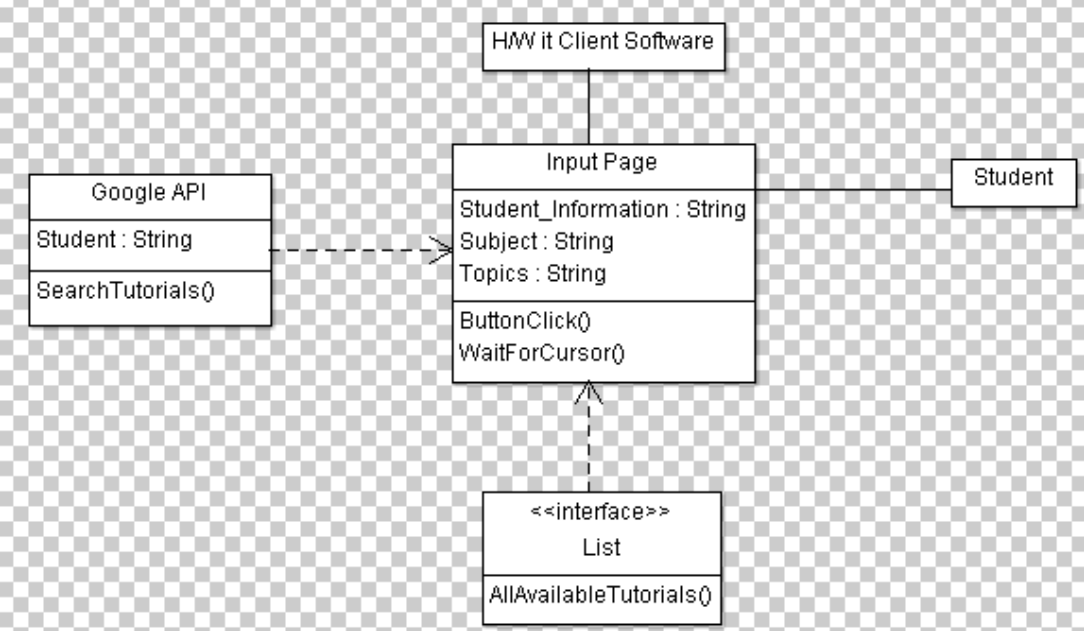
\includegraphics[height=6.0 cm,width=10.0 cm]{class.png}
\caption{Class Diagram}
\end{figure}
\hspace*{0.3in}Class Diagram is a type of static structure diagram that describes the structure of a system by showing the systems classes, their attributes, and the relationships between the classes. Class diagrams are the backbone of almost every object oriented methods, including UML. They describe the static structure of a system .
\subsection{Data Objects and Relationships}

\begin{figure}[h]
\centering
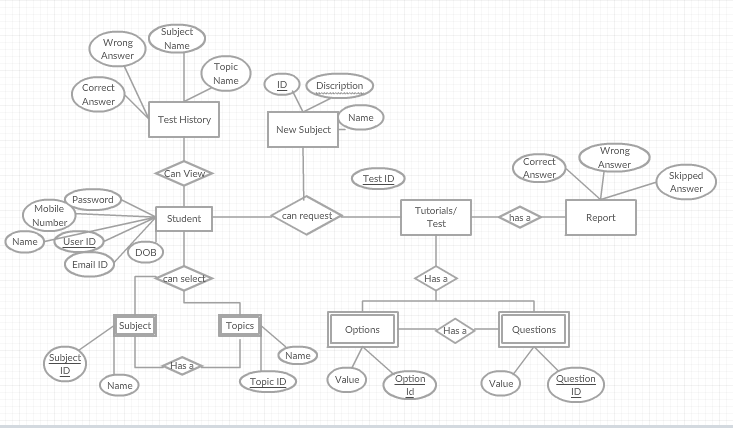
\includegraphics[height=7.0 cm,width=14.0 cm]{er.png}
\caption{E-R Diagram}
\end{figure}

\newpage
\section{FUNCTIONAL MODEL AND DESCRIPTION}

\subsection{Data Flow Diagram}
\begin{figure}[!h]
DFD Level 0\\
\\
\centering
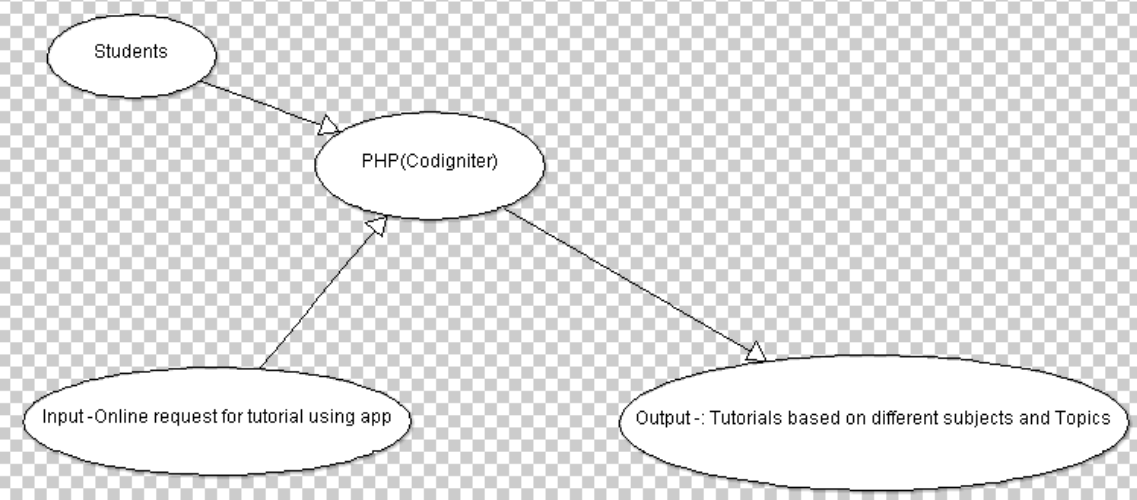
\includegraphics[height=6cm,width=12cm]{dfd0.png}
\caption{Data Flow Diagram Level 0}
\end{figure}

\begin{figure}[!h]
DFD Level 1\\
\\
\centering
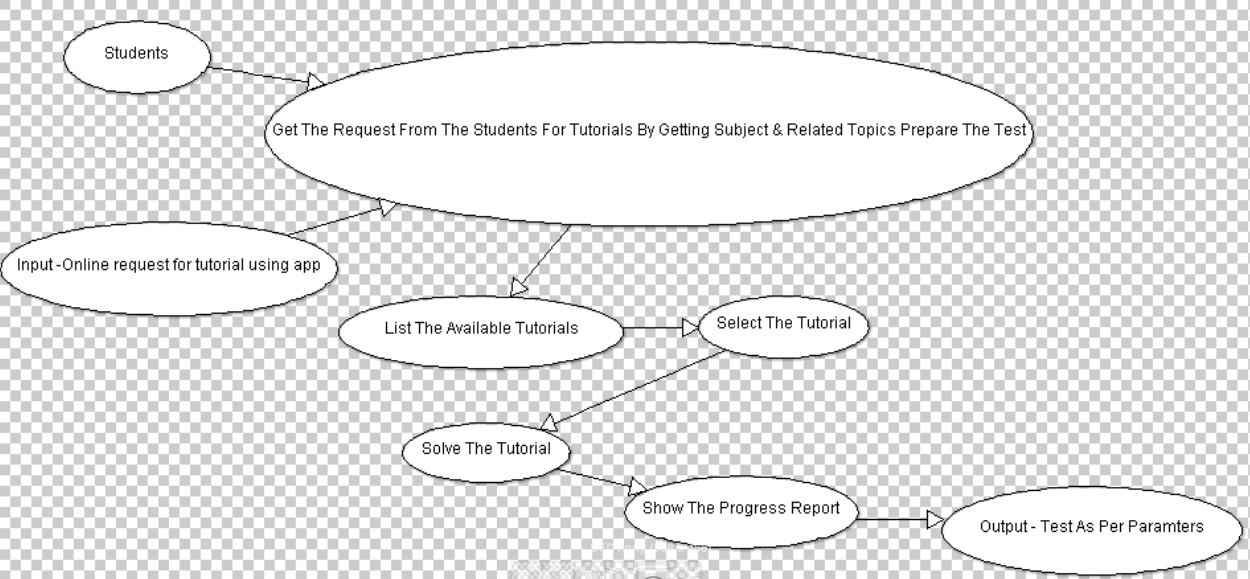
\includegraphics[height=6cm,width=12cm]{dfd1.png}
\caption{Data Flow Diagram Level 1}
\end{figure}
\\
\newpage
\subsubsection{Activity Diagram}
\begin{figure}[!h]
\centering
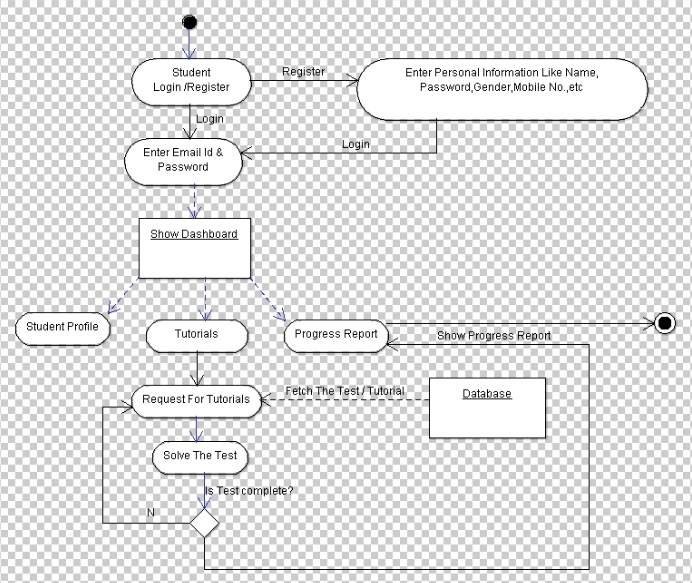
\includegraphics[height=7cm,width=8cm]{activitystudent.png}
\caption{Activity diagram for student}
\end{figure}
\\
\begin{figure}[!h]
\centering
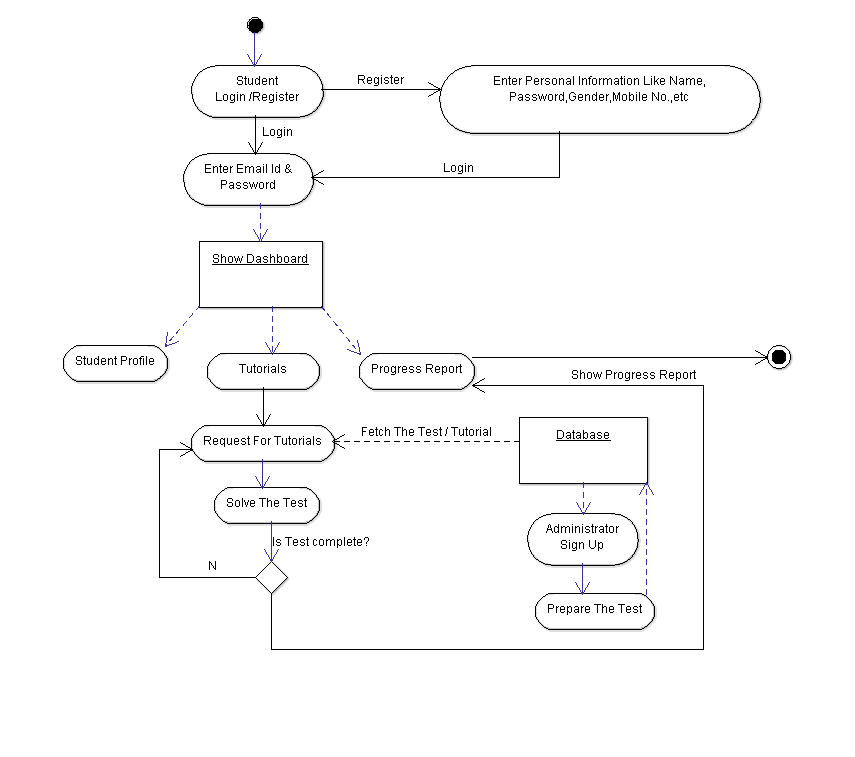
\includegraphics[height=7cm,width=7.5cm]{activity_admin.png}
\caption{Activity diagram for admin}
\end{figure}
\\


\subsection{Non Functional Requirements} 
\hspace{0.3in}In each project,in addition to serving end user goals we must serve the needs of the development team.Non functional requirements are the properties that the product must have. These are the characteristics or qualities that make the product attractive,or usable,or fast,or reliable.Non functional requirements do not alter product's functionality.\\
\textbf{Non Functional requirements}
\begin{itemize}
\item Interface Requirements
\item Performance Requirements
\item Software quality attributes such as availability [ related to Reliability],
modifiability [includes portability, reusability, scalability] , performance,security
\end{itemize}
\subsection{Sequence Diagram}
\begin{figure}[!h]
\centering
\includegraphics[height=9cm,width=10cm]{sequence.png}
\caption{Sequence Diagram}
\end{figure}
\\

\chapter{DETAILED DESIGN DOCUMENT USING APPENDIX A AND B}
\newpage
\section{INTRODUCTION}

\subsection{Purpose}
\hspace*{0.3in}This document describes the high level design for data, architecture, interface and components for the software. It highlights the detailed design of the system including of architectural design, component level design, data design and interface design. Also the issues, constraints and limitations are discussed.\\

\subsection{Scope}
\hspace*{0.3in}We using fully functional full stack framework t make learning easy and paperless  .

\section{ARCHITECTURAL DESIGN}
\\
\subsection{System Architecture}

\begin{figure}[!h]
\centering
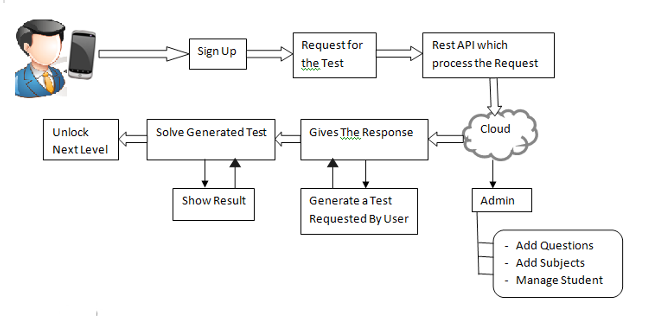
\includegraphics[height=6 cm,width=10 cm]{arch.png}
\caption{System Architecture}
\end{figure}

\section{COMPONENT DESIGN}

\subsection{Class Diagrams}
\\

\subsubsection{Package diagram}
\\
\begin{figure}[!h]
\centering
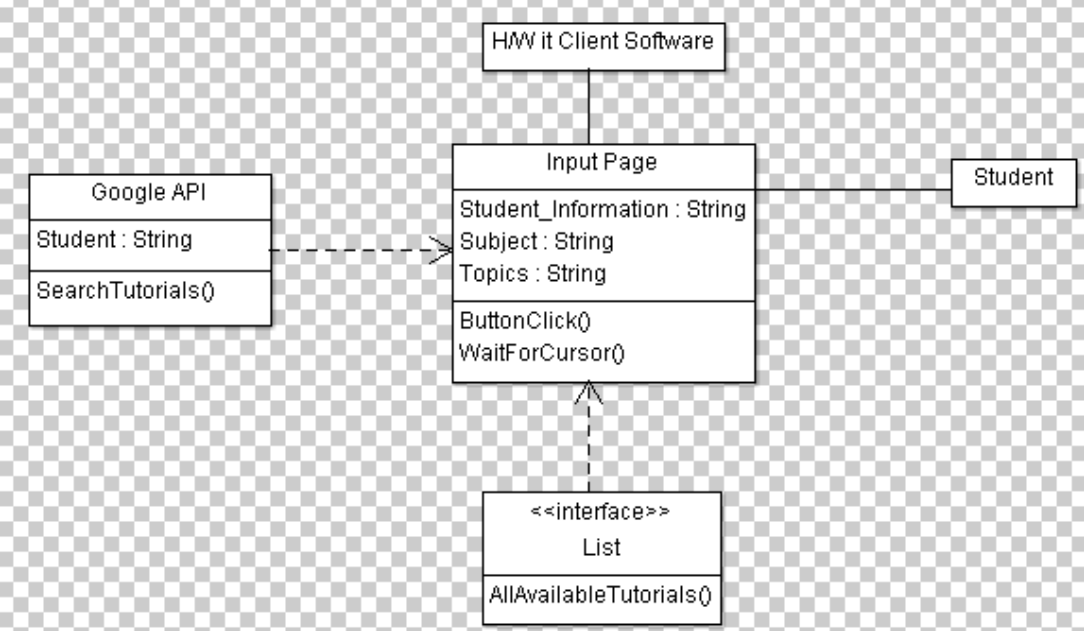
\includegraphics[height=6cm,width=7cm]{class.png}
\caption{Package diagram}
\end{figure}
\subsubsection{Deployment Diagram}
\\
\begin{figure}[!h]
\centering
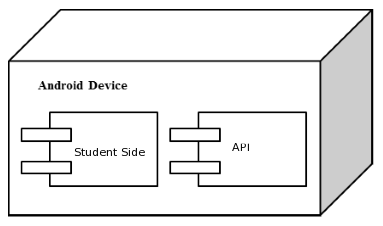
\includegraphics[height=4.5cm,width=7cm]{Deployment.png}
\caption{Deployment Diagram}
\end{figure}
\\
 
 
\chapter{PROJECT IMPLEMENTATION}
\newpage
\section{INTRODUCTION}
This document describes both the test plan and the test procedure along with goals and objectives of test specifications.\\

\section{Goals and Objectives}
The objective of our test plan is to find and report as many bugs as possible to improve the integrity of the system. Although exhaustive testing is not possible, a broad range of tests is exercised to achieve the goal of bug free and accurate results in software.\\

\section{TOOLS AND TECHNOLOGIES USED}
\begin{itemize}
\item Filezilla\\
FileZilla is a free software, cross-platform FTP application, consisting of FileZilla Client and FileZilla Server. Client binaries are available for Windows, Linux, and macOS, server binaries are available for Windows only. The client supports FTP, SFTP and FTPS (FTP over SSL/TLS).\\
FileZilla's source code is hosted on SourceForge and the project was featured as Project of the Month in November 2003.[3] However, there have been criticisms that SourceForge bundles malicious software with the application; and that FileZilla stores users' FTP passwords insecurely.
\item Sublime Text\\
Sublime Text is a sophisticated text editor for code, markup and prose.
Sublime Text is a proprietary cross-platform source code editor with a Python application programming interface (API). It natively supports many programming languages and markup languages, and functions can be added by users with plugins, typically community-built and maintained under free-software licenses.
\item Postman
A Little About Postman. Postman is a Google Chrome app for interacting with HTTP APIs. It presents you with a friendly GUI for constructing requests and reading responses

\end{itemize}
\newpage

 
\chapter{SOFTWARE TESTING}
\newpage
\section{Statement of Scope}
The software testing is to be done for all components in every module of software.The results of the modules must be compared with actual known values to test the correctness of the procedure.\\
\\
\textbf{Introduction:}Software testing is the process of executing a program or system with the intent of finding errors.
\begin{figure}[h]
\centering
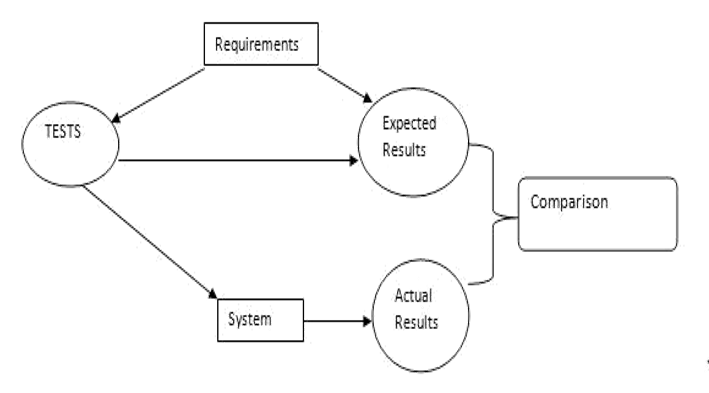
\includegraphics[height=3.5 cm,width=10 cm]{testing.png}
\caption{Basic Testing Mechanism}
\end{figure}
\section{TEST PLAN}
\hspace*{0.3in}This section describes the overall testing strategy and the dissertation management issues that are required to properly execute effective tests.
\subsection{Testing Strategy}
The overall strategy for software testing is described here.
\subsection{Unit Testing}
\hspace*{0.3in}Each module is tested separately.The criterion selected for unit test modules are identity modules that have core functionality implemented and its execution is independent of other modules.\subsection{Integration Testing}
\hspace*{0.3in}In integration testing, the modules which are unit tested are combined and testing is performed to see if the correct information is passed between the modules as per the algorithms..
\subsection{Static and Dynamic Analysis}
\hspace*{0.3in}Static analysis involves going through the code in order to find out any possible defect in the code. Dynamic analysis involves executing the code and analysing the output.
\subsection{GUI Testing}
\hspace*{0.3in}The user interface is tested to check the functionality of all the scenes, buttons and navigation components.
\subsection{White Box Testing}
\hspace*{0.3in}White box testing strategy deals with the internal logic and structure of the code. White box testing is also called as glass, structure, open box or clean box testing.
\subsection{Black Box Testing}
\hspace*{0.3in}Black Box Testing is testing without knowledge if internal working of the item being tested. For Example when black box testing is applied to software engineering, the tester would only know the legal input and what the excepted output should be, but not how the program actually arrive at those output.
\subsection{Test Schedule}
The work products gives correct flow of the system and produced its intended function.
\subsection{Test Case}
\hspace*{0.3in}A test case in software engineering is a set of conditions or variables under which a tester will determine whether an application or software system is working correctly or not.\\
\begin{table}[h]
\centering
\begin{tabular}{|p{0.7in}|p{0.7in}|p{1.2in}|p{0.8in}|p{0.8in}|p{0.5in}|}
\hline	  
Test Case ID  & Test Case Name &Test Case \newline Descripton &Expected Results &Actual \newline Results &Test Status
\\
\hline	  
IC1  & Admin Login &To check \newline wheather the \newline application gives access to authorised person &Access is \newline given to \newline Authorized user only & Access is \newline given to \newline Authorized user only&Passed
\\
\hline	
IC2 &	Student Login &	To check \newline wheather the \newline application gives access to student&	Access is \newline given to \newline Student	& Access is \newline given to \newline Student &	Passed

\\
\hline	  
IC3	& SignUp & To check  \newline wheather new \newline user is added	& New user \newline added sucessfully &	New user \newline added sucessfully	& Passed  
\\
\hline	  
IC4	& Student Details modification at admin side	& To check  \newline wheather students details is insert , delete , or update	& Student details modified &	Student details modified &	Passed
\\
\hline	  
IC5 &	Subject Module &	To check \newline wheather new \newline subject and \newline subtopics added	& Subject added sucessfully &	Subject added sucessfully	 & Passed
\\
\hline	  
IC6 &	Question Module &	To check\newline wheather new \newline question is  \newline added as well as edited & Question added sucessfully & Question added sucessfully & Passed
\\
\hline	  
IC7 &	Test Module  &	To check \newline wheather \newline requested  \newline test is \newline generated	& Test generated sucessfully &	Test generated successfully	 & Passed
\\
\hline	  
IC8 &	Report Module &	To check \newline wheather correct \newline report is \newline genereted	& Report generated sucessfully &	Report generated successfully	 & Passed
\\

\hline
\end{tabular}
\caption{Test Plan}
\end{table}

\begin{table}[h]
\cntering
\begin{tabular}{|p{0.7in}|p{0.7in}|p{1.2in}|p{0.8in}|p{0.8in}|p{0.5in}|}
\hline	  
IC9 &	User Profile &	To check \newline wheather user \newline profile is \newline created and edited	& User profile created sucessfully & User profile created successfully & Passed
\\
\hline	  
IC10 &	Notification Module &	To check \newline wheather notification \newline is send & Notification send successfullyy &	Notification send successfully	 & Passed
\\
\hline	  
IC11 &	In app Updates &	To check \newline wheather updates\newline are send & Updates send successfully &	Updates send successfully	 & Passed
\\
\hline	  
IC12 &	Subject  Request &	To check \newline wheather subject \newline is sent & Subject request is successfully created &	Subject request is successfully created	 & Passed
\\
\hline	  
IC13 &	Toppers module &	To check \newline wheather \newline toppers \newline are listed \newline or not & Toppers are displayed sucessfully &	Toppers are displayed successfully	 & Passed
\\
\hline	  
IC14 &	Test History &	To check \newline wheather test\newline history is \newline displayed & Test history displayed sucessfully &	Test history displayed sucessfully	 & Passed
\\

\hline	  
IC15 &	LeaderBoard Module &	To check \newline wheather \newline LeaderBoard \newline is displayed & LeaderBoard displayed successfully &	LeaderBoard displayed successfully	 & Passed
\\
\hline
\end{tabular}
\caption{Test Plan}
\end{table}




\\    
   
\chapter{Results}
\newpage
\section{User Interface}
\hspace*{0.3in} The features of a computer system which allows the user to interact with it. A user interface, also sometimes called a human-computer interface, comprises both hardware and software components. It handles the interaction between the user and the system. ... graphical user interface (GUI).\\
\subsection{Web Application}
\begin{figure}[!h]
\centering
\includegraphics[height=6.0 cm,width=10.0 cm]{home.png}
\caption{Home Screen}
\end{figure}
\\
\begin{figure}[!h]
\centering
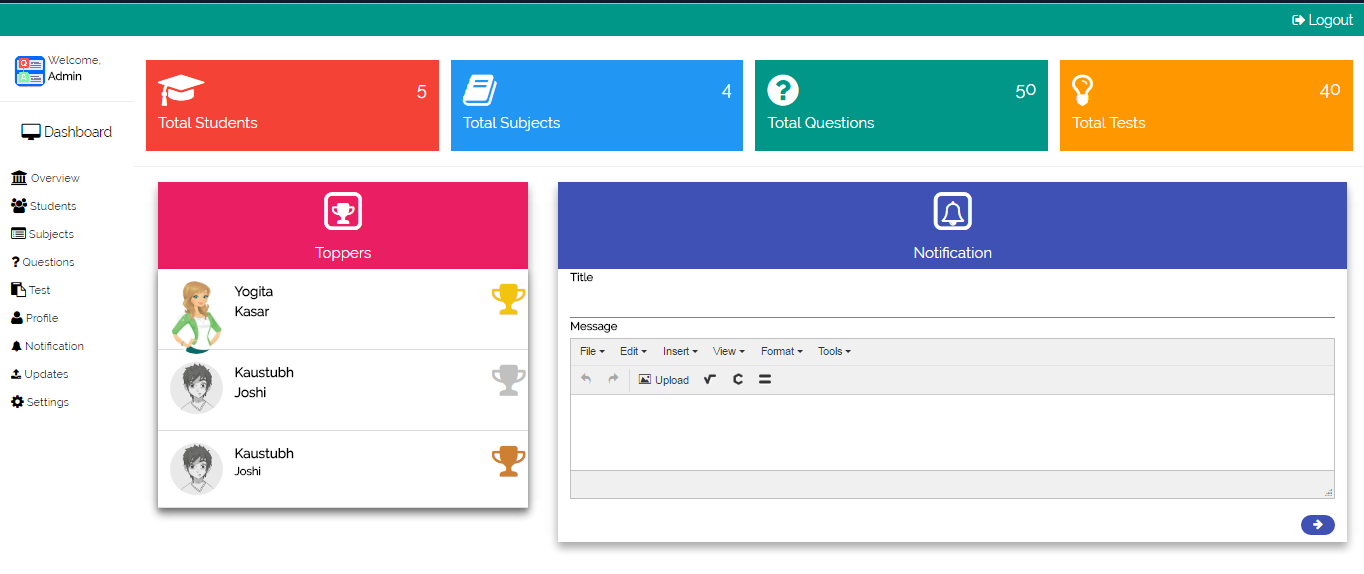
\includegraphics[height=6.0 cm,width=10.0 cm]{dash.png}
\caption{Dashboard}
\end{figure}
\\

\begin{figure}[!h]
\centering
\includegraphics[height=5.0 cm,width=10.0 cm]{stud.png}
\caption{Student Module}
\end{figure}
\\
\newpage
\begin{figure}[!h]
\centering
\includegraphics[height=5.0 cm,width=10.0 cm]{sub.png}
\caption{Subject Module}
\end{figure}
\\
\begin{figure}[!h]
\centering
\includegraphics[height=5.0 cm,width=10.0 cm]{report.png}
\caption{Report Module}
\end{figure}
\\
\subsection{Android Application}
\begin{figure}[!h]


\includegraphics[height=7.5 cm,width=4.0 cm]{login.png}
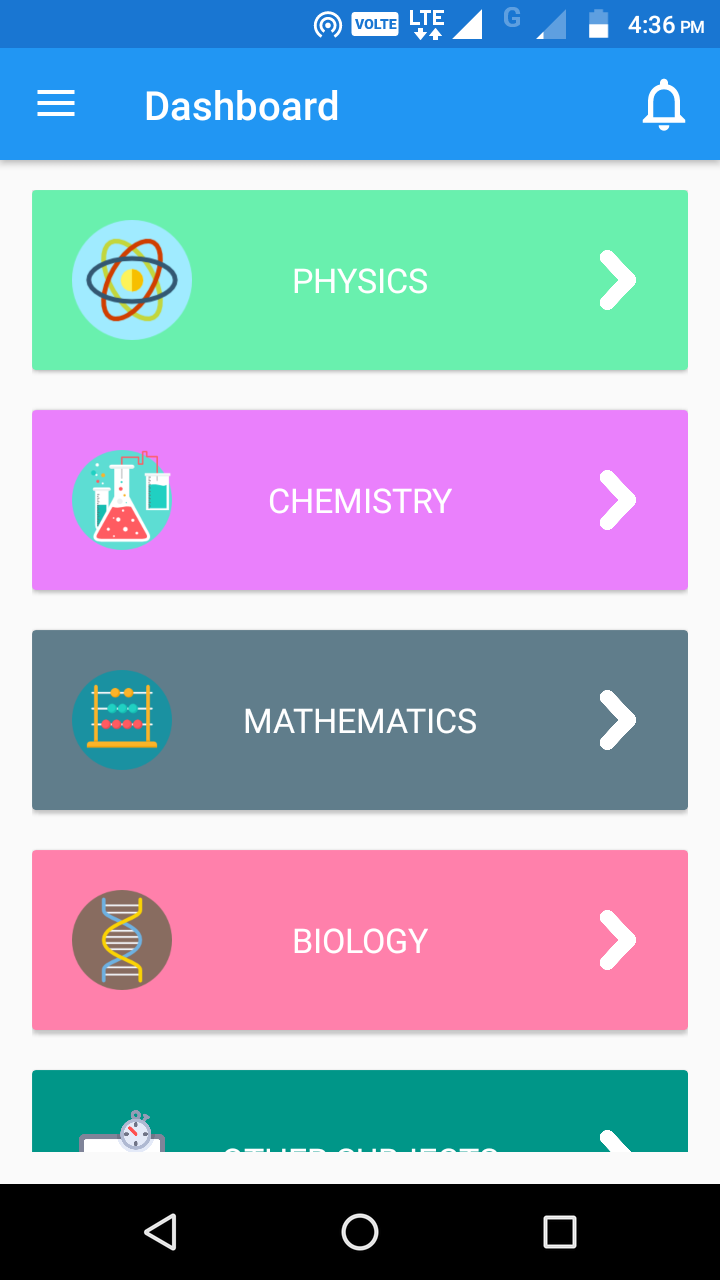
\includegraphics[height=7.5 cm,width=4.0 cm]{dasha.png}
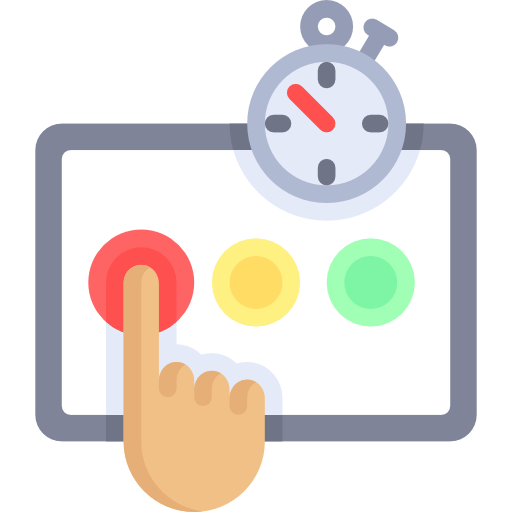
\includegraphics[height=7.5 cm,width=4.0 cm]{test.png}
\caption{login Module , Dashboard Module , Test Module}

\end{figure}
\begin{figure}[!h]
\centering
\includegraphics[height=7.5 cm,width=4.0 cm]{testreport.png}
\includegraphics[height=7.5 cm,width=4.0 cm]{testhistory.png}
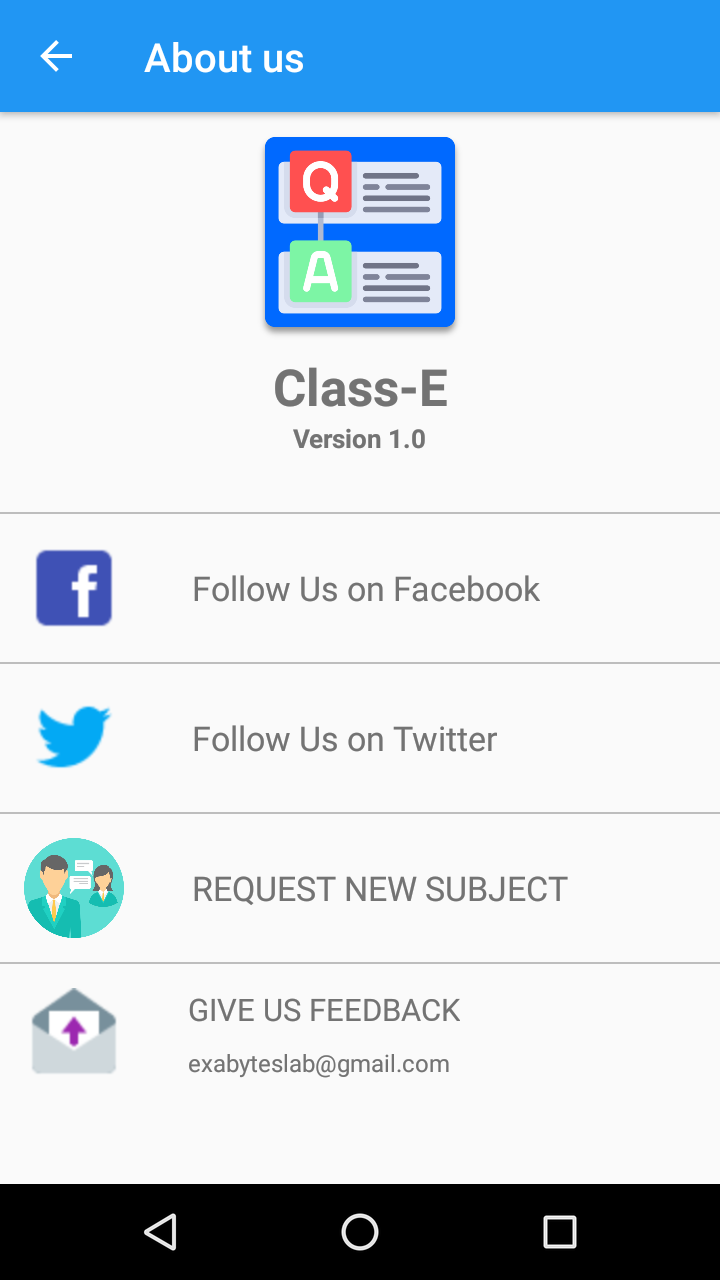
\includegraphics[height=7.5 cm,width=4.0 cm]{about.png}
\caption{Test Report , Test History , About Module}

\end{figure}
\\

 
\chapter{DEPLOYMENT AND MAINTENANCE}
\newpage
\section{INSTALLATION AND UN-INSTALLATION}

\textbf{Pre-Installation}
\begin{enumerate}
\item Make sure that your android device should have required storage space to install app.
\item android device should connected with internet
\end{enumerate} 

\textbf{Installation Instructions}
\begin{enumerate}
\begin{itemize}
\item Open the Google Play Store app . Note: you can also go to play.google.com.

\item Search or browse for Class-E Android app.
 
\item Tap Install 

\item Follow the onscreen instructions to complete process and get the content.


\end{itemize}



\end{enumerate} 

\newpage



     
\chapter{CONCLUSION AND FUTURE SCOPE}
\newpage
\hspace*{0.3in}
In this project, we have presented a Android Based E-Learning Application .We implement the  system through an application on Android platform. And to illustrate the effectiveness of the system, we develop admin site  using Codigniter.\\
 We also conduct several experiments to evaluate our application.  The experimental
results show that our developed system can work effectively on android devices.  Friendly user interface is very  important  for  an  application.   Most  of  people  decide  whether  to  use an application only by its user interface.  Thus, we use bootstrap and w3.css to design admin site .\\
proposed system is developed which is accessible at any time as long as
the user brings the mobile devices and internet connection is available.
System is developed using bootstrap for the mobile device in which it is
supported with javascript and CSS as its basic display that can be used
for further needs.
\\ 

\bibliographystyle{plain}

\bibliographystyle{ieeetr}
%\bibliography{biblo}

\begin{appendices}
\begin{thebibliography}{99}
%\addcontentsline{toc}{chapter}{Bibliography}

\bibitem{bm} Scripting queries https://www.google.co.in
\bibitem{bm} Stack Overflow https://stackoverflow.com/ 
\bibitem{bm} Codeigniter : https://www.codeigniter.com 
\bibitem{bm} Bootstrap : getbootstrap.com/ 
\bibitem{bm} Slack : https://exabyteslab.slack.com/
\bibitem{bm} Android Hive : www.androidhive.info/
\bibitem{bm} www.viralandroid.com
\bibitem{bm} https://getmdl.io/ 
\bibitem{bm} https://www.w3schools.com/w3css/

\bibitem{bm} “Mobile-Based Learning Design with Android Development Tools” 2014 1st International Conference on Information Technology, Computer and Electrical Engineering (ICITACEE)

\bibitem{bm} M. L. Crescente and D. Lee, “Critical issues of m-learning: Design models, adoption processes, and futur00e trends,” J. Chinese Inst. Ind. Eng., vol. 28, no. 2, pp. 111–123, 2011.

\bibitem{bm} X. Zhao, X. Wan, and T. Okamoto, “Adaptive content delivery in ubiquitous learning environment,” in Proc. 6th IEEE WMUTE, 2010, pp. 19–26.

\bibitem{bm} “Design of a Microlecture Mobile Learning System Based on Smartphone and Web Platforms” ,IEEE TRANSACTIONS ON EDUCATION, VOL. 58, NO. 3, AUGUST 2015

\end{thebibliography}



\chapter{LABORATORY ASSIGNMENTS ON PROJECT ANALYSIS OF ALGORITHM DESIGN}
\newpage
\begin{itemize}
\textbf{\ Problem feasibility using concepts of knowledge canvas and IDEAMatrix}\\

\textbf{Feasibility:}\\
\textbf{Knowledge Canvas:}\\ 
\hspace*{0.3 in} Knowledge canvas is one that depicts the knowledge forces and knowledge flow across the organization. It captures the current knowledge state and knowledge forces in the environment. It tries to build the bigger and broader knowledge scenario for you and your environment. It is simple representation of knowledge opportunities with reference to the environment.\\
	
\textbf{IDEA Matrix:}\\
\hspace*{0.3 in} This framework identifies the key parameters to be enhanced for creating knowledge value for systemic knowledge innovation.\\
\begin{figure}[!h]
\centering
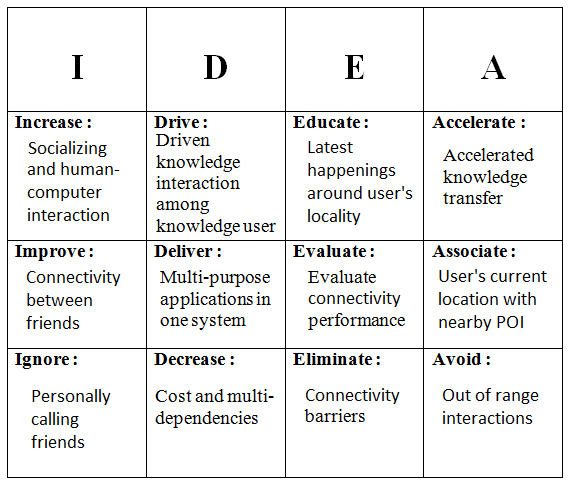
\includegraphics[height=10.0 cm,width=12.0 cm]{idea.png}
\caption{Idea Matrix}
\end{figure}
\\





\chapter{LABORATORY ASSIGNMENTS ON PROJECT QUALITY AND RELIABILITY TESTING OF PROJECT DESIGN}
\newpage

\hspace*{0.3in}It should include assignments such as\\ 
\begin{itemize}
\item
Use of divide and conquer strategies to exploit distributed/parallel/concurrent
processing of the above to identify object, morphisms, overloading in
functions (if any), and functional relations and any other dependencies
(as per requirements). It can include Venn diagram, state diagram, function
relations, i/o relations; use this to derive objects, morphism, overloading
\item
Use of above to draw functional dependency graphs and relevant Software
modeling methods, techniques including UML diagrams or other
necessities using appropriate tools.
\item
Testing of project problem statement using generated test data (using
mathematical models, GUI, Function testing principles, if any) selection
and appropriate use of testing tools, testing of UML diagram’s reliability.
Write also test cases [Black box testing] for each identified functions. You can use Mathematica or equivalent open source tool for
generating test data.
\item 


\end{itemize}


\textbf{Testing of Project Problem Statement}\\

\textbf{Introduction:} Software testing is the process of executing a program or system with the intent of finding errors. Or it involves any activity aimed at evaluating an attribute or capability of the system and determining that it meets its required results. Software is unlike other physical processes where inputs are received and outputs are produced. Where software differs is in that manner in which it fails. Most physical systems fail in a fixed set of ways. By contrast, software can fail in bizarre ways. Detecting all of the different failure modes for software is generally infeasible.\\ 
\\
\hspace*{0.3 in}Testing is performed for following purposes:\\ 
\hspace*{0.3 in}1. To improve quality\\
\hspace*{0.3 in}2. Verification and validation Basic software testing \\
\\
\chapter{PROJECT PLANNER}
\newpage
\begin{itemize}

\item Slack
\\
Slack brings team communication and collaboration into one place so you can get more work done, whether you belong to a large enterprise or a small business. Check off your to-do list and move your projects forward by bringing the right people, conversations, tools, and information you need together. Slack is available on any device, so you can find and access your team and your work, whether you’re at your desk or on the go.

\begin{figure}[h]
\centering
\includegraphics[height=3.5 cm,width=7.0 cm]{slack.png}
\caption{Slack}
\end{figure}
\item Github
\\
GitHub is a development platform inspired by the way you work. From open source to business, you can host and review code, manage projects, and build software alongside millions of other developers.
\begin{itemize}
\item Code security

\item Access controlled

\item Hosted where you need it

\begin{figure}[h]
\centering
\includegraphics[height=3.0 cm,width=8.0 cm]{git.png}
\caption{Git Hub}
\end{figure}
\end{itemize}
\end{itemize}


\chapter{REVIEWERS COMMENTS OF PAPER SUBMITTED}
\newpage
\begin{enumerate}
\item Paper Title: Android Based E-Learning Application “Class-E”
\item Name of the Conference/Journal where paper submitted : International Research Journal of Engineering and Technology (IRJET)
\item Paper accepted/rejected : Accepted
\item Review comments by reviewer : Paper Accepted Successfully
\item Corrective actions if any : No
\end{enumerate}

\chapter{PLAGIARISM REPORT}
\newpage
Plagiarism report
\begin{center}
	\begin{figure}[!htbp]
		\centering
		\fbox{\includegraphics[width=250pt]{pla.png}}
	  \caption{Plagiarism Report}
	  \label{fig:Plagiarism Report}
	\end{figure}
\end{center} 


\chapter{TERM-II PROJECT LABORATORY ASSIGNMENT}
\newpage
\includepdf [pages={1-4}]{IRJET.pdf}
\newpage

\includepdf [pages={1-4}]{certificates.pdf}
\chapter{INFORMATION OF PROJECT GROUP MEMBERS}
\newpage
\begin{enumerate}
\item \textbf{Name :} Joshi Kaustubh Ajay.
\hspace{60 mm}\includegraphics[width=60pt]{kk.png}
\item \textbf{Date of Birth :} 13/6/1996
\item \textbf{Gender :} Male
\item \textbf{Permanent Address : }N-35/S-4/7/1/2, Swami Vivekanand  Nagar , Cidco,Nashik-422009.
\item \textbf{E-Mail :} exabytes.js@gmail.com
\item \textbf{Mobile/Contact No. :} 9762720307
\item \textbf{Placement Details :} Placed at Solace Infotech Nashik..
\item \textbf{Paper Published :} Yes 
\end{enumerate}

\newpage
\begin{enumerate}
\item \textbf{Name :} Kasar  Yogita Hemraj \hspace{60 mm}\includegraphics[width=60pt]{yy.png}
\item \textbf{Date of Birth :} 28/01/1994
\item \textbf{Gender :} Female
\item \textbf{Permanent Address :} N-53 V.G.-25/5 Patil nagar, Cidco,Nashik-422009.
\item \textbf{E-Mail :} yogitakasar156@gmail.com
\item \textbf{Mobile/Contact No. :} 9960136918
\item \textbf{Placement Details : }Placed at Netwin Info Solutions, Nashik.
\item \textbf{Paper Published :} Yes 
\end{enumerate}

\newpage
\begin{enumerate}
\item \textbf{Name :} Mahajan Mayuri Vinod \hspace{60 mm}\includegraphics[width=60pt]{mm.png}
\item \textbf{Date of Birth :} 01/04/1996
\item \textbf{Gender :} Female
\item \textbf{Permanent Address :} N-32/R-3/40-5 Vruindavan Chowk,Cidco,Nashik-9
\item \textbf{E-Mail :}mayurimahajan1496@gmail.com
\item \textbf{Mobile/Contact No. :} 8668449846
\item \textbf{Placement Details :} Placed at Deskera, Pune.
\item \textbf{Paper Published :} Yes 


\end{enumerate}

\newpage
\begin{enumerate}
\item \textbf{Name :} Nikam Pooja Ganesh \hspace{60 mm}\includegraphics[width=60pt]{pp.png}
\item \textbf{Date of Birth :} 29/09/1995
\item \textbf{Gender :} Female
\item \textbf{Permanent Address :} N-52/A-D/2 9/7 Saibaba nagar,New Cidco,Nashik-422009.
\item \textbf{E-Mail :} pujanikam2329@gmail.com
\item \textbf{Mobile/Contact No. :} 8605903136
\item \textbf{Placement Details :} Placed at Solace Infotech, Nashik.
\item \textbf{Paper Published :} Yes 


\end{enumerate}
\end{appendices}


\end{document}
